\documentclass[a4paper]{article}
\usepackage{afterpage}
\usepackage{caption}
\usepackage{subcaption}
\usepackage{hanging}
\usepackage{setspace}
\usepackage[a4paper, margin=1.2in, footnotesep=1.5\baselineskip]{geometry}
\usepackage[
backend=biber,
style=chem-biochem,
citestyle=nature,
url=false,
doi=true,
isbn=false,
autocite=superscript
]{biblatex}
\usepackage{todonotes}
\usepackage{doi}
\usepackage{titlesec}
\usepackage{hyperref}
\usepackage{caption}
\usepackage{subcaption}
\usepackage{pdflscape}

\renewcommand{\thefootnote}{\alph{footnote}}
%\newcommand{\sectionbreak}{\clearpage}
\renewcommand*{\bibfont}{\footnotesize}
\addbibresource{../references.bib}
\urlstyle{rm}
  
\hypersetup{
    colorlinks=true,
    citecolor=magenta,
    linkcolor=magenta
}

\setlength{\parskip}{0.75em}

\onehalfspacing

\pagestyle{plain}

\graphicspath{ {./figures/} }

\renewcommand{\abstractname}{Summary}

\title{
	{\normalsize Doctoral Confirmation Report} \\
	{\LARGE \textsc{Building Resilience: How do Species Interactions Shape Ecosystem Collapse?}}
}
\author{
  {\large Fernando Cagua}
}
\date{}

\begin{document}

\maketitle







\section*{Introduction}

The present report summarises the advances made since the presentation of the PhD proposal in August 2015. The literature review and the description of the research, including the planned methodology and analysis techniques has already been included in the PhD proposal and will not be expanded here (the PhD proposal is attached to this report). Here I focus on presenting the results obtained to date. To date there have not been changes on the scope or the research objectives, neither on the methodology or the proposed timeline.

Natural ecosystems provide important services---like food and water---we humans depend on to a large extent.
  Much like the failure of a single key financial institution can trigger unexpected crashes on the stock market, human pressures---such as biological invasions and species extinctions---can cause sudden collapses that severely transform the way ecosystems function.
  However, despite its importance, we do not completely understand the dynamics that make ecosystems resilient to collapse.
  Because the functioning of ecosystems is largely determined by the network of interactions between the species that inhabit them, my proposed research aims to quantify the role played by species interactions in determining the resilience of ecosystems.
  To achieve this, I will focus on networks of mutually beneficial interactions, like those between plants and their pollinators, and use a combination of empirical data, computer simulations and ecological theory.
  Ultimately I want to understand why, when and how ecosystem collapses occur, and how to recover from them.

\section*{PhD objectives}

The overall objective of my proposed research is to quantify the role played by species interactions in modulating ecosystem resilience. 
To do so, I will focus on the network of mutualistic interactions between plants and pollinators \autocite{Bascompte2006, Bascompte2007, Klein2007}.
These networks, which form the base of pollination systems, play a globally important role in the maintenance of biodiversity and crop production \autocite{Bascompte2007, Klein2007}.

I will focus on empirically informed theoretical approaches.
Throughout my thesis, I will use computer simulated communities to estimate the population dynamics of the species in the community, and then I will directly quantify stability properties from fluctuations in the species populations \autocite{Bastolla2009, Garcia-Algarra2013}.
I will develop these `synthetic` communities under a wide range of parameters to answer the specific questions I aim to answer in each chapter of my dissertation.

In the first chapter of my thesis I will concentrate on biotic invasions.
Specifically I have a twofold objective: first, I aim to determine which network characteristics shape the its resistance and resilience to invasions, and second to determine how biotic invasions reshape network resistance and resilience by affecting existing interactions in the community.

Remarkably, invaded pollination communities have been shown to have structures that support more species \autocite{Stouffer2014} and can be more robust than those of un-invaded communities \autocite{Albrecht2014}.
Indeed we know which structures can enhance biodiversity \autocite{Bastolla2009} and delay the onset of catastrophic collapses \autocite{Lever2014}, but there are still serious mismatches between theoretical predictions and empirical observations.
I argue that this can be at least partially explained by the interplay between the degree of redundancy among species in the network and the apparent facilitation and competition between species in a mutualistic network.
Therefore, the objective of my second chapter is to evaluate the effects that structural redundancy has on the stability of ecological networks.

The aim of my third chapter is to obtain useful lessons for ecosystem management from a direct analysis the network structure.
Ecosystems are complex, non-linear systems that are very difficult to control.
On the other hand, recent work in theoretical physics has highlighted that is indeed possible to regulate them using targeted interventions \autocite{Cornelius2013}.
I propose to build upon these findings to determine the optimal set of management actions---from both a theoretical and a feasibility perspective---that are required to modify an ecosystem state.






\section*{Progress}

As specified on the PhD proposal schedule, I have started by the third objective of my thesis. However a thorough literature review and a outline of the research methodology has already been completed for Objectives 1 and 2. This can be found in the attached Research Proposal document. 

\begin{itemize}
	\item Objective 3: Controlling ecosystems for resilience management
	\begin{itemize}
		\item Objective 3.1. Determine the set of driver species: To date I have analised previously published data, and obtained preliminary results. An initial draft of the paper is underway. 
		\item Objective 3.2. Determine which interventions on the driver species are necessary to guide the ecosystem to the desired state: Ecosystem models are being currently developed by Jenny Shang, an intern under the University of Canterbury Summer Reserach Scholarship Programme. Results for this component are expected by mid February.
	\end{itemize}
\end{itemize}

\subsection*{Objective 3.1: Determining driver species in pollination networks}
 
\subsubsection*{Introduction}

Ecological communities are formed by the interconnection of several species. Therefore, changes in the abundances of one species can potentially alter the abundances of the species they interact with. For instance, in a classic example of ecosystem cascades, a reduction on the abundance of sea otters, an important predator or sea urchins, can drive a dramatic reduction on kelp abundances because the sea urchins that consume kelp are released from predation. It has been long established that some species, like the sea otter, have a disproportionate large effect in their environment relative to their abundance. 

In several ecosystems the relative importance of species have been identified based on empirical observations of long term dynamics. However, in less studied, highly diverse, or where the "keystone" role is shared by several species, it can be challenging to determine which is the set of species that influence the most the ecosystem dynamics. Alternative approaches that recognize a continuum of importance and that are less dependent on empirical observations have also been developed. Some of them are based on metrics that evaluate their position in the food web or on mass balance models of functional groups. Nevertheless, these approaches are conceptually limited to throphic interactions and in general ignore the structural mechanisms that allow or prevent the spread of perturbations in the ecosystem.

From a systems perspective, perturbations like over-exploitation, eutrophication or global warming are equivalent to management actions like culling, no-take areas or captive rearing in the sense that they have the potential to modify the abundances of one or several species in the ecosystem. Therefore identifying these key species is crucial not only to predict how these perturbations will spread trough the community but also to guide effective conservation efforts.

Recent work on the control of complex systems suggest that in principle it is possible to alter any ecological community's composition, by modifying the abundances of just some key species \autocite{Isbell2013, Cornelius2013}. Here, we apply these theories to estimate the controllability of different ecological communities and to find driver species: species, that due to the structural characteristics of their interactions are more likely to drive the dynamics of the community.

Invasive species have been shown to have a disproportionate effect on the structure of pollination communities. Influencing for example the strength of species interactions, and the degree of network nestedness and connectivity \autocite{Olesen2002, Aizen2008, Bartomeus2008, Vila2009, Traveset2013}. However whether this influcence is translated into a driver role has not been tested. mHere we use plant pollinator communities to investigate the number of species that should be managed to control population dynamics of the whole community, the characteristics that determine wheter a species should be managed or not and how invasive species fit. 

\subsubsection*{Methodology} 

To investigate the dynamic controllability of pollination networks, we used ten paired plants-pollinator communities. Each par was composed by a community invaded by a plant and a community free of the invasive species. Weighted visitation networks were constructed from previously published visitation data collected from pollination communities in Bristol, Great Britain \autocite{Lopezaraiza-Mikel2007} and the National Cap de Creus in Northeastern Spain \autocite{Bartomeus2008}. The four British uninvaded communities the non-invaded plots were obtained by experimentally removing the invasive species \textit{Impatients grandulifera} (\hyperref[fig:photographs]{Figure \ref{fig:photographs}a}). Contrastingly, Spanish uninvaded communities were obtained from plots that were not been colonised by the invasive species \textit{Carpobrotus affine acinaciformis} or \textit{Opuntia stricta} (\hyperref[fig:photographs]{Figure \ref{fig:photographs}b, c}). In each of the networks we calculated the minimum number of driver species---species that need to be managed in order to gain full control of the community.

\begin{figure}
    \centering
    \begin{subfigure}{0.3\textwidth}
        \centering
        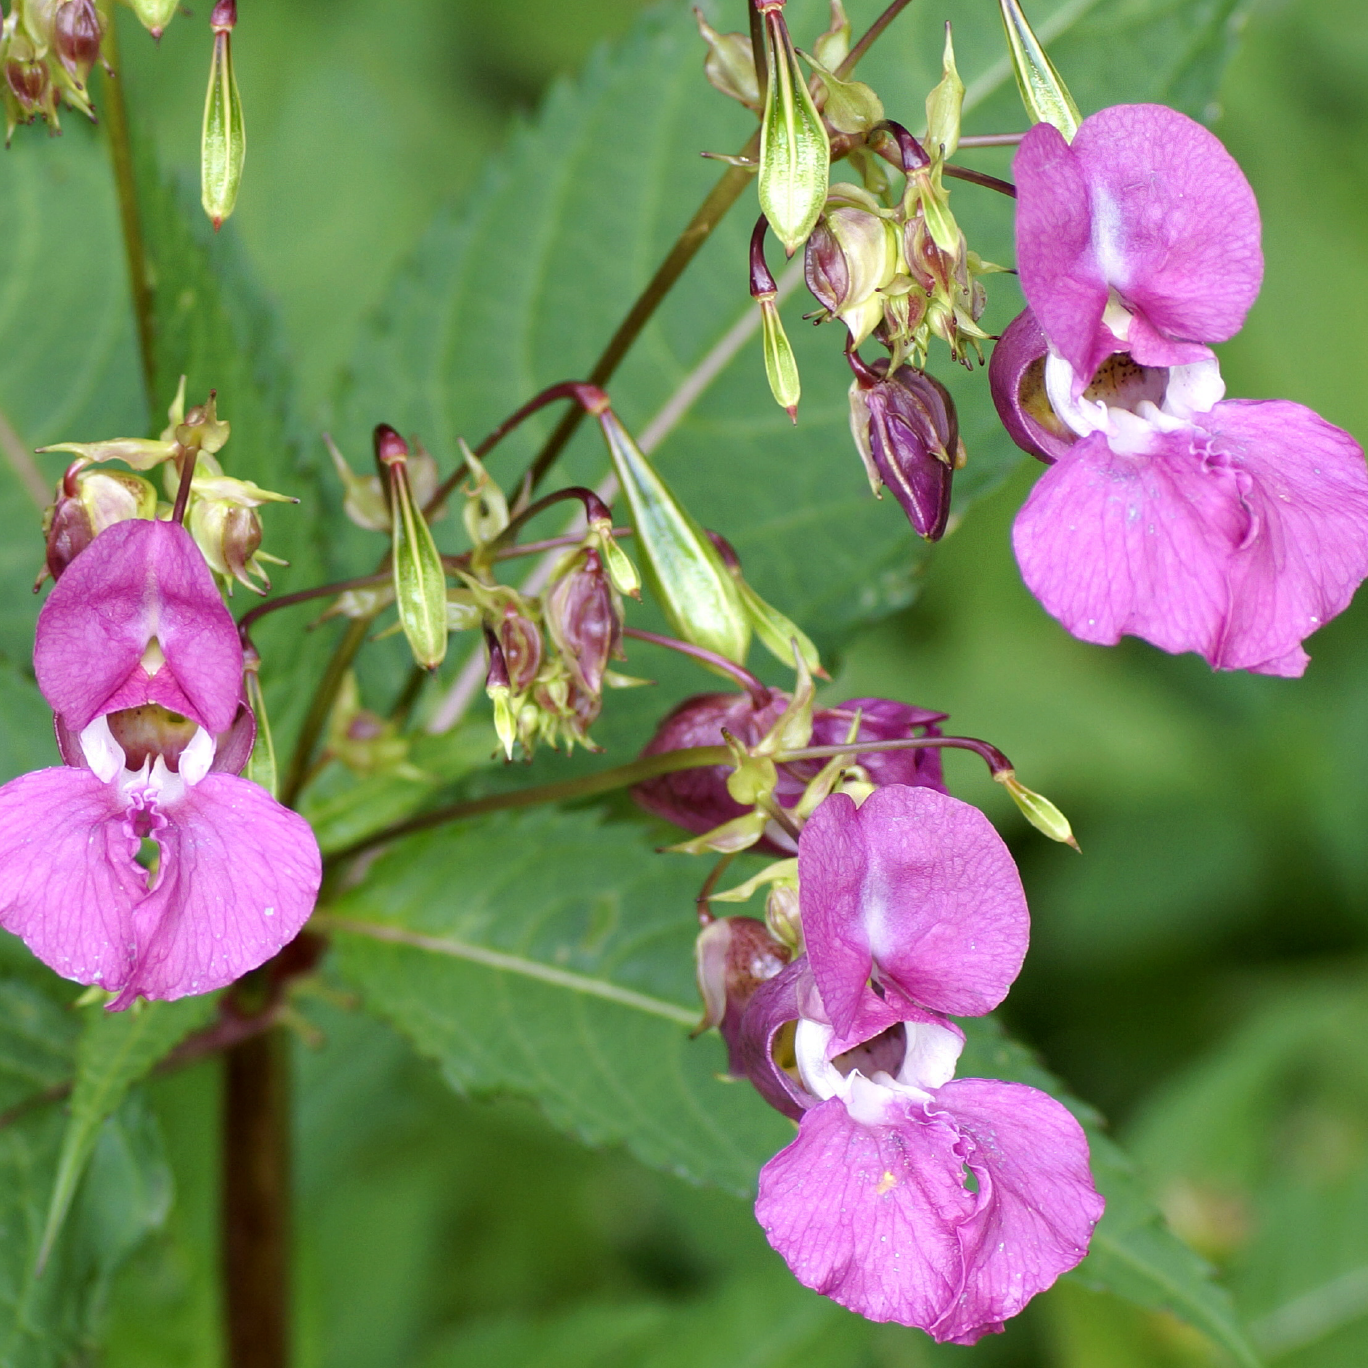
\includegraphics[width=\textwidth]{Impatiens_glandulifera}
        \caption{\textit{Impatiens glandulifera}}
    \end{subfigure}
    \hfill
    \begin{subfigure}{0.3\textwidth}
        \centering
        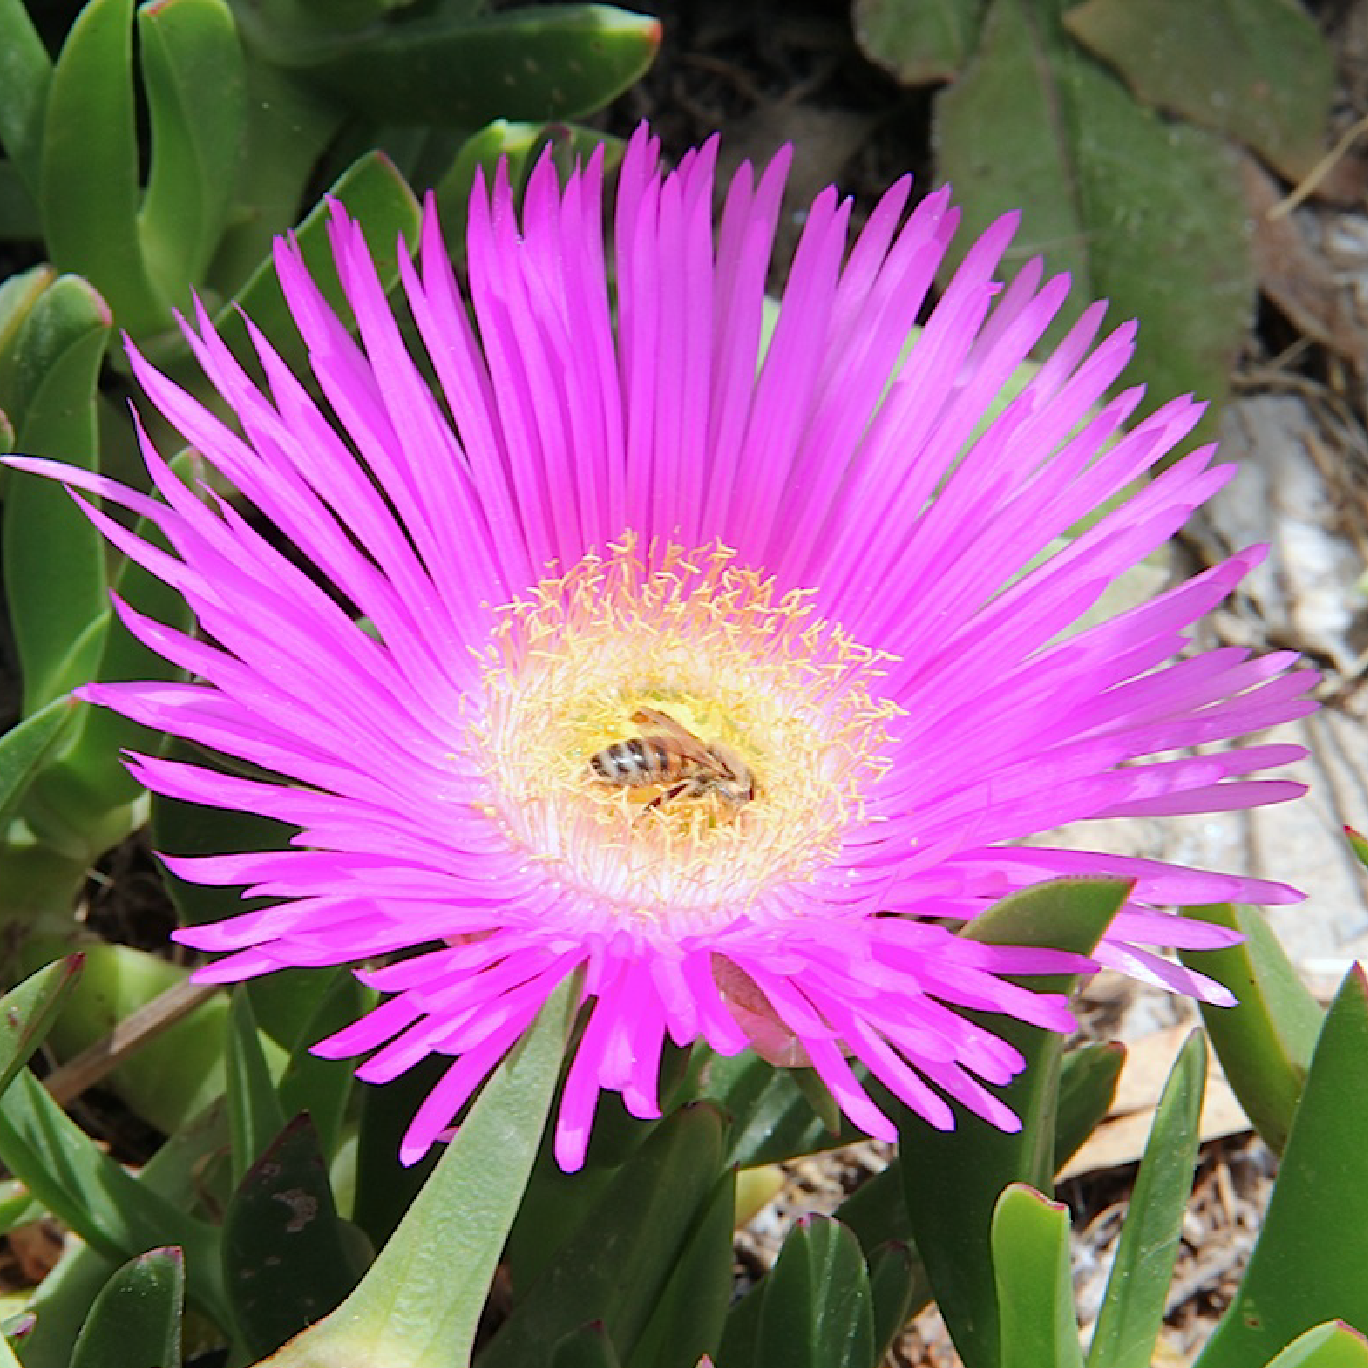
\includegraphics[width=\textwidth]{Carpobrotus_acinaciformis}
        \caption{\textit{Carpobrotus acinaciformis}}
    \end{subfigure}
    \hfill
    \begin{subfigure}{0.3\textwidth}
        \centering
        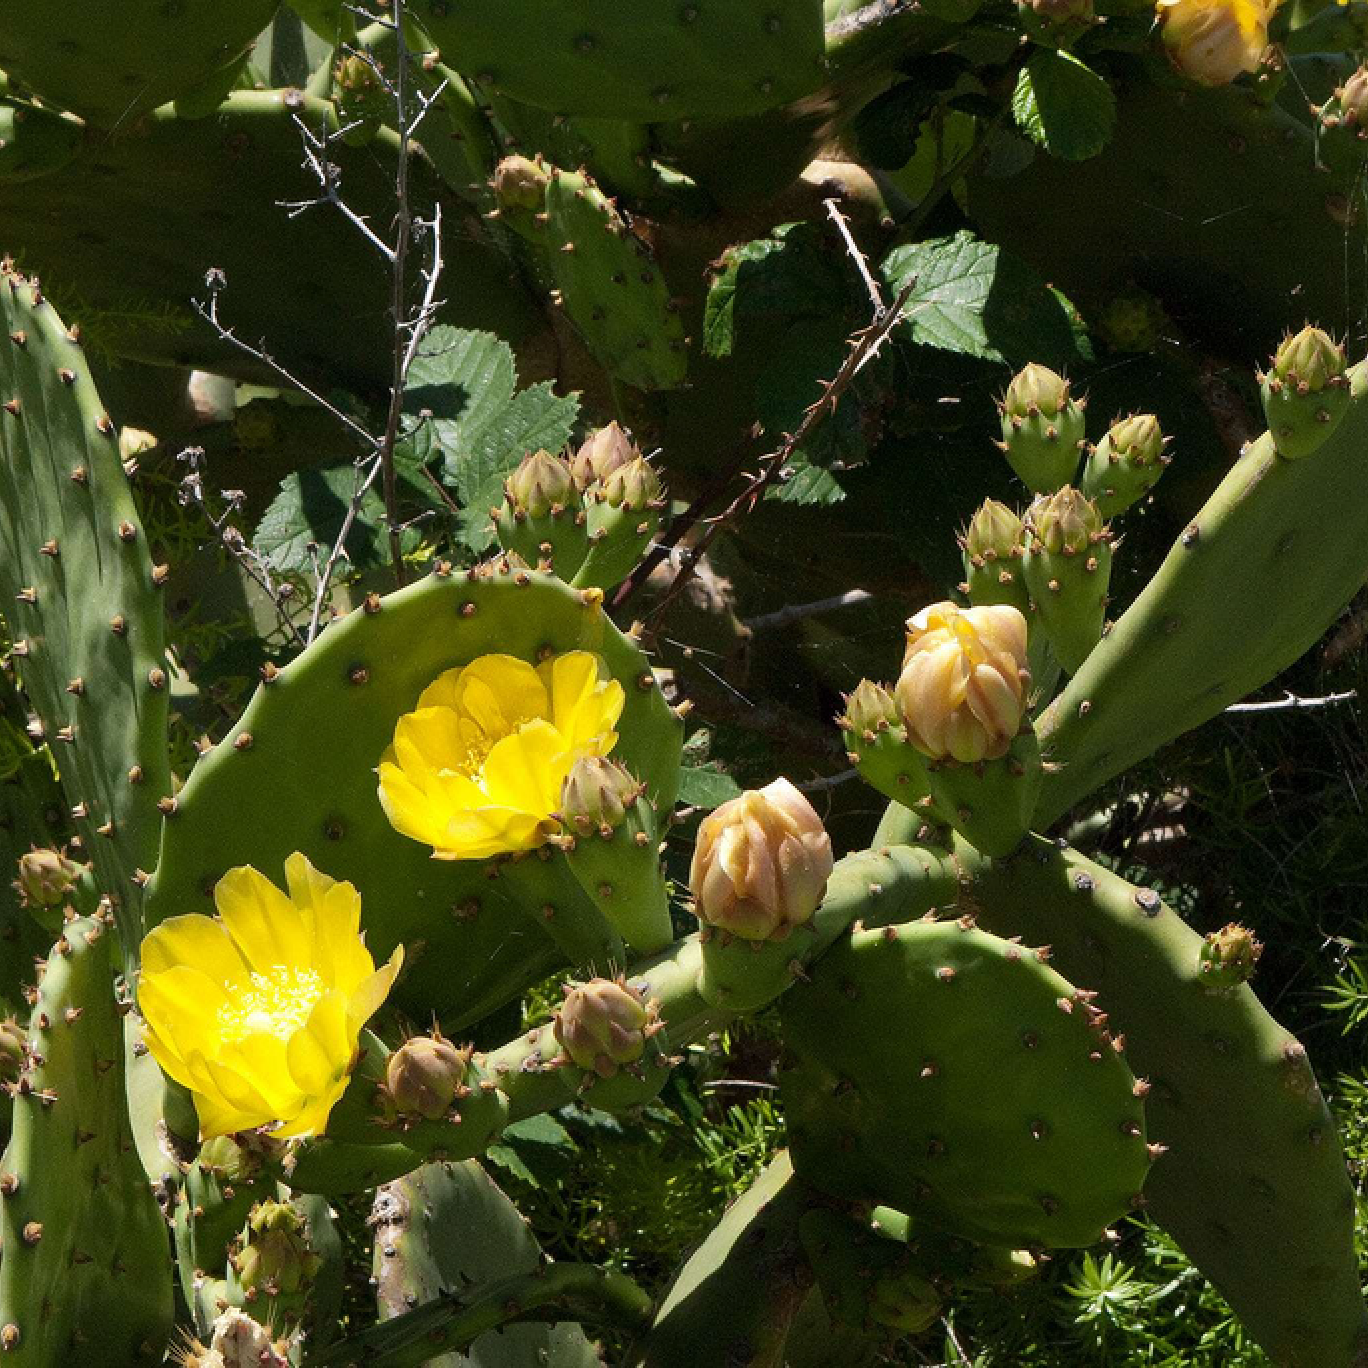
\includegraphics[width=\textwidth]{Opuntia_stricta}
        \caption{\textit{Opuntia stricta}}
    \end{subfigure}
    \hfill
    \caption{
    Invasive species present in the studied pollination communities (photographs by \href{https://commons.wikimedia.org/wiki/File:Impatiens_glandulifera_Royle_(7677070626).jpg}{Udo Schmidt}, \href{https://commons.wikimedia.org/wiki/File:Carpobrotus_acinaciformis_pm.jpg}{Peter Mansfeld}, and \href{https://www.flickr.com/photos/tony_rodd/5265326818}{Tony Rodd}).
    }
    \label{fig:photographs}
\end{figure} 

We first assigned a direction to each link between plants and pollinators given by the direction of dependency. For each link between a plant and its polinator we quantified the level of dependency of the plant on the pollinator and visceversa \autocite{Bascompte2006}. The link points to the plant if the its dependency on the pollinator is larger than the pollinator's dependency on the plant. The dependency of plant $i$ on pollinator $j$ is the ratio between the visits comming from pollinator $j$ and allpollinator visits to plant $i$. The dependency of pollinator $j$ on plant $i$ is the ratio of the visits by pollinator $j$ to plant $i$ and all visits of pollinator $j$. 

In a directed network, a matching is a subset of links in which no two links share a common starting species or a common ending species. A species is matched if it is an ending node of an link in the matching. Otherwise, it is unmatched. It has been shown that the number of driver species can be calculated by counting the number of unmatched nodes in the directed graph representation of the pollination network \autocite{Liu2011}. We then found a maximum in the an alternative bipartite representation of the pollination network \autocite{Csardi2006} (\autoref{fig:maximum_matching}). 

\begin{figure}
    \centering
    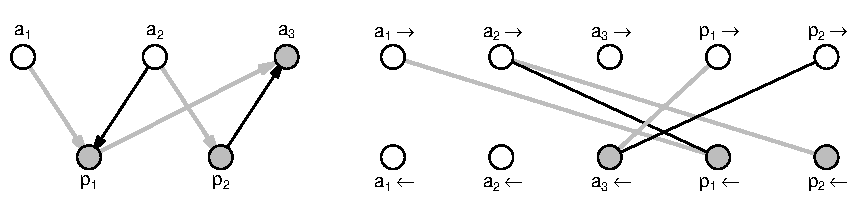
\includegraphics[width=\textwidth]{control_net}
    \caption{
    On the left a simple pollination network; the direction of the arrows indicates the direction of the largest dependency between species pairs. On the right the representation of the network used to calculate the maximum matching (in blue). Matched species, i.e. those whose dynamic could be ``controled'' by another species are shown in blue. Note that the maximum matching is not necessarely unique.
    }
    \label{fig:maximum_matching}
\end{figure} 

We calculated dependencies based on visitation frequency, which has been shown to be an appropiate surrogate of the interspecific effects \autocite{Bascompte2006, Vazquez2005}. However, because the degree distribution, and ultimately the number of driver species, can be affected by the sampling method \autocite{Bluthgen2010} we compared the number of driver species in a pollination community in which both visitation frequency and effectiveness were measured \autocite{Ballantyne2015}.

To quantify to what extent the number of driver species is characteristic of the structure of pollination networks we compared them a suit of random null-models. A set of null models were based on network randomisations that mantained the degree of plants, pollinators, and both plants and pollinators. To analyse the effects of the chosen directionality, we devised a null model in which we randomised the visitation patterns and re-calculated the new dependencies. 

We quantified the relative importance of each species for network dynamics. To do this, we counted the number of times a particular species was a driver species across all possible maximum matchings in the pollination network. The number of maximum matchings were found by generating the line graph of the alternative bipartite network representation (\autoref{fig:maximum_matching}), and then enumerating the maximal cliques in the complement of the line graph \autocite{Csardi2006}. 

Finally, we asked the question wheter some structural properties can predict the relative importance of driver species. We regressed the importance of each species against measures of centrality (degree, betweeness), measures related to network robustness (contribution to nestedness) and measures of strength of association (visitation levels). 

\subsubsection*{Preliminary results} 


\section*{Research Plan}

So far dates estimated in the proposal research plan have been 

\subsubsection*{Schedule:}
%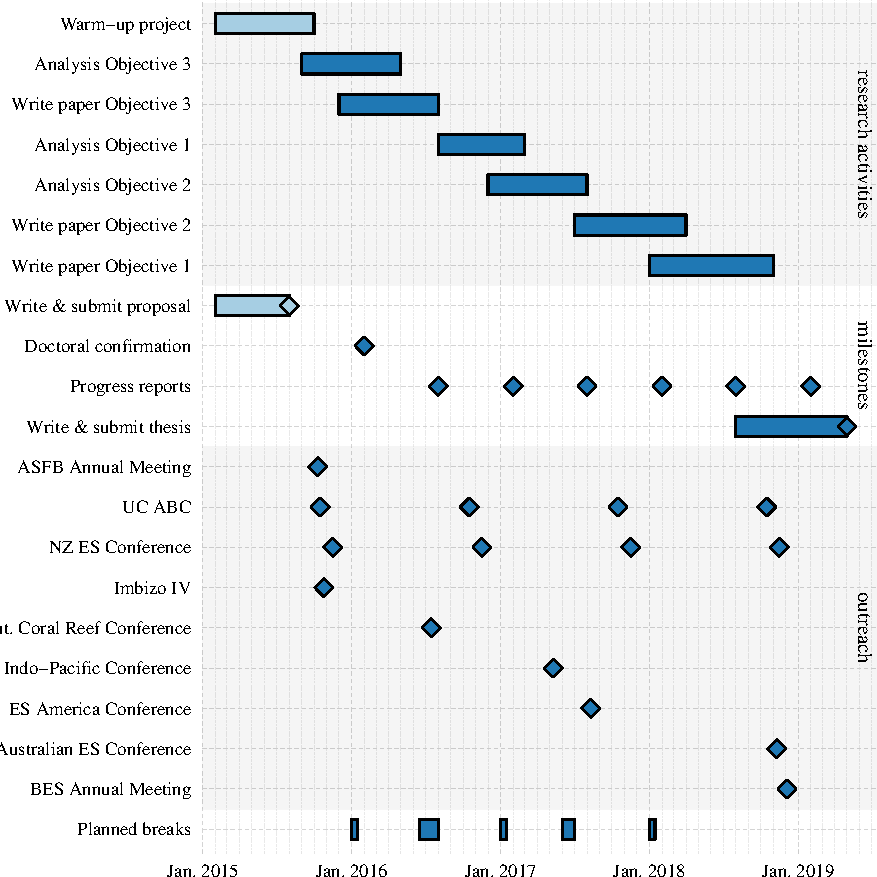
\includegraphics{schedule}
 
\printbibliography

\end{document}
